
%\documentclass[draft]{beamer}
\documentclass{beamer}

\usetheme{Singapore} 
\usepackage{graphicx}
\usepackage{verbatim}
\usepackage{natbib}
\usepackage{bm}
\usepackage{movie15}
\usepackage{xmpmulti}


\title{NARCCAP and netCDF}
\author{Adam Wilson}
\date{\today}
%\setbeamersize{text margin left=6mm, text margin right=2mm} 
  
\begin{document}

\begin{comment}
\section{NARCCAP}
\frame{
  \frametitle{North American Regional Climate Change\\ Assessment Program}
  \begin{center} 
    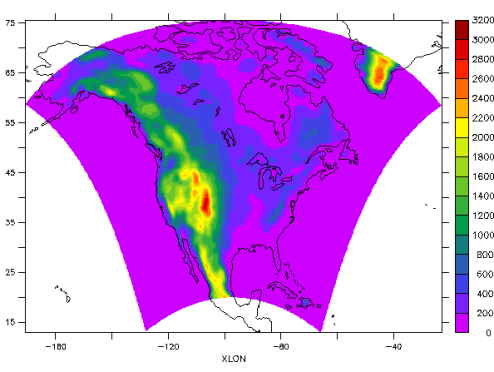
\includegraphics[width=.5\textwidth]{narccap-domain.png}\\ 
\url{http://www.narccap.ucar.edu/}
  \end{center}
}

\frame{
  \frametitle{NARCCAP}
Sponsored by
\begin{itemize}
\item NCAR (National Center for Atmospheric Research)
\item NOAA (National Oceanic and Atmospheric Administration)
\item NSF (National Science Foundation)
\item USDOE  (U.S. Department of Energy)
\item EPA  (U.S. Environmental Protection Agency)
\item OURANOS (a Canadian consortium on regional climatology and adaptation to climate change)
\end{itemize}
}

\end{comment}

\frame{
  \frametitle{NARCCAP Priorities}
  Focus on uncertainty across models (rather than across scenarios) 
 \begin{center} 
    \uncover<2>{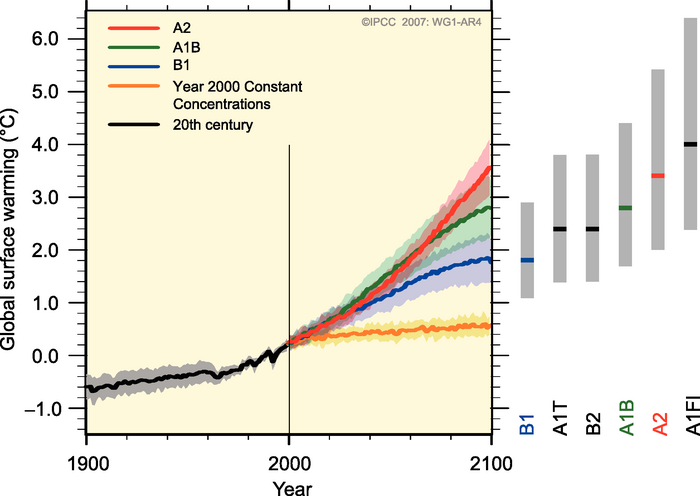
\includegraphics[width=.6\textwidth]{figure-spm-5-l.png}
   \end{center}
  All NARCCAP data are from the A2 emissions scenario}
}

\frame{
  \frametitle{NARCCAP Priorities}
  Focus on uncertainty across models (rather than across scenarios) 
  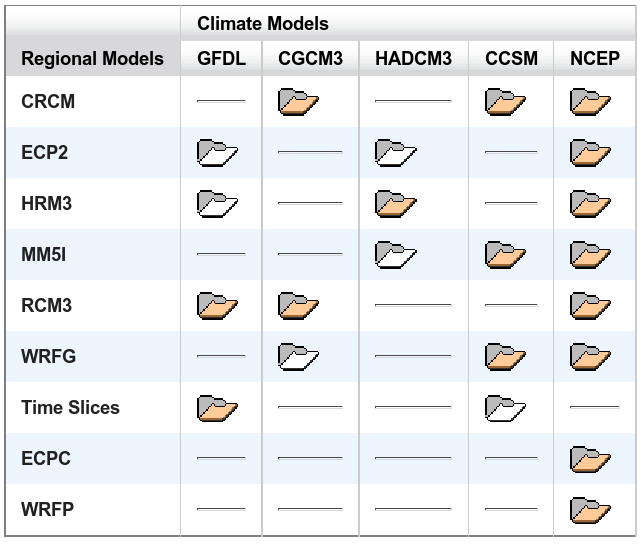
\includegraphics[width=.6\textwidth]{NARCCAP_data.png}
}
 
\frame{
  \frametitle{Lab Exercise}
 \begin{enumerate}
\item {Download monthly mean GCM (GFDL) data from the IRI Data Library}
\item {Explore the NARCCAP site to see how their data is organized,
    then download subsetted data from the course website}
\item {Use Panoply to explore netCDF files}
\item {Use Climate Data Operators (CDO) from within R to process the monthly and
    daily data to annual and seasonal metrics}
\item {Read data into R and make a few plots}
\end{enumerate}
}

\section{netCDF}
\frame{
  \frametitle{What is netCDF (network Common Data Form)?}
  ... software libraries and machine-independent data formats
  that support the creation, access, and sharing of {\bf array-oriented
  scientific data}. 
    \uncover<2>{
      \begin{center} 
        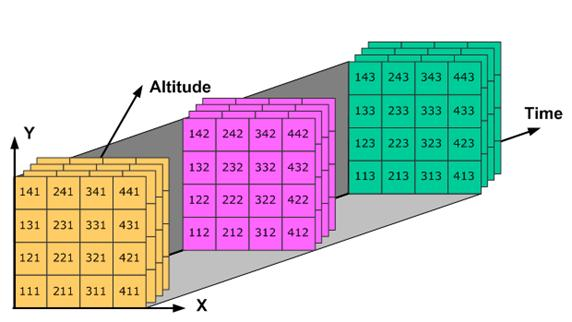
\includegraphics[width=.6\textwidth]{netcdf.jpg}
      \end{center}}
      \begin{itemize}
      \item Developed at Unidata UCAR \url{www.unidata.ucar.edu/software/netcdf/}
      \end{itemize}
}

\frame{
  \frametitle{What is netCDF (network Common Data Form)?}
 \begin{itemize}
     \item  {Self-Describing. { \color{gray}\small{A netCDF file includes information about the data it contains.}}}
     \item  {Portable. {\color{gray}\small{A netCDF file can be accessed by computers with different ways of storing integers, characters, and floating-point numbers.}}}
     \item {Scalable. {\color{gray}\small{A small subset of a large dataset may be accessed efficiently.}}}
     \item {Appendable. {\color{gray}\small{Data may be appended to a properly structured netCDF file without copying the dataset or redefining its structure.}}}
     \item {Sharable. {\color{gray}\small{One writer and multiple readers may simultaneously access the same netCDF file.}}}
     \item {Archivable. {\color{gray}\small{ Access to all earlier forms of netCDF data will be supported by current and future versions of the software.}}}
 \end{itemize}
}

\frame{
  \frametitle{What's in a netCDF?}
 \begin{itemize}
\item {Dimensions \color{gray}{ latitude, longitude, time (height/depth)}}
\item {Variables  \color{gray}{ name, type, shape, attributes and values}}
\item { Attributes  (``metadata'')  \color{gray}{information about names, dimensions, units, and type (numeric,
    character, etc)}}
\end{itemize}
}

\begin{frame}[fragile]
\tiny
\begin{verbatim}
netcdf file:/media/Data2/Data/narccap/pr_RCM3_gfdl_1968010103.nc
 dimensions:
   time = UNLIMITED;   // (8760 currently)
   bnds = 2;
   yc = 104;
   xc = 134;
 variables:
   double time_bnds(time=8760, bnds=2);
    float pr(time=8760, yc=104, xc=134);
     :grid_mapping = "Transverse_Mercator";
     :standard_name = "precipitation_flux";
     :long_name = "Precipitation";
     :units = "kg m-2 s-1";
     :coordinates = "lon lat";
     :missing_value = 1.0E20f; // float
      :_FillValue = 1.0E20f; // float
    double time(time=8760);
     :long_name = "time";
     :standard_name = "time";
     :axis = "T";
     :calendar = "noleap";
     :units = "days since 1968-01-01 00:00:0.0";
   double lat(yc=104, xc=134);
     :units = "degrees_north";
     :long_name = "latitude";
     :standard_name = "latitude";
     :axis = "Y";
 :title = "UC Santa Cruz RegCM3 model output prepared for NARCCAP
          present-day climate using NCEP/DOE Reanalysis";
 :experiment_id = "present-day climate using NCEP/DOE Reanalysis";
 :table_id = "Table 2";
 :project_id = "NARCCAP";
 :source = "RegCM3 (2006) atmosphere: RegCM3v3.1 hydrostatic, split-explicit, 
            horizontal equal area grid resolution of 50 km by 50 km
 :institution = "CCIL, UC Santa Cruz (Climate Change and Impacts Laboratory, 
            University of California, Santa Cruz, CA, USA)";

\end{verbatim}
\end{frame}

\end{document}